
\documentclass[border=10pt, 12pt]{standalone}
\usepackage[svgnames]{xcolor}
\usepackage{amsmath}
\usepackage{pgfplots}
\pgfplotsset{compat=newest}
\usepackage[sfdefault]{FiraSans}
\usepackage{FiraMono}
\renewcommand*\familydefault{\sfdefault}
\begin{document}
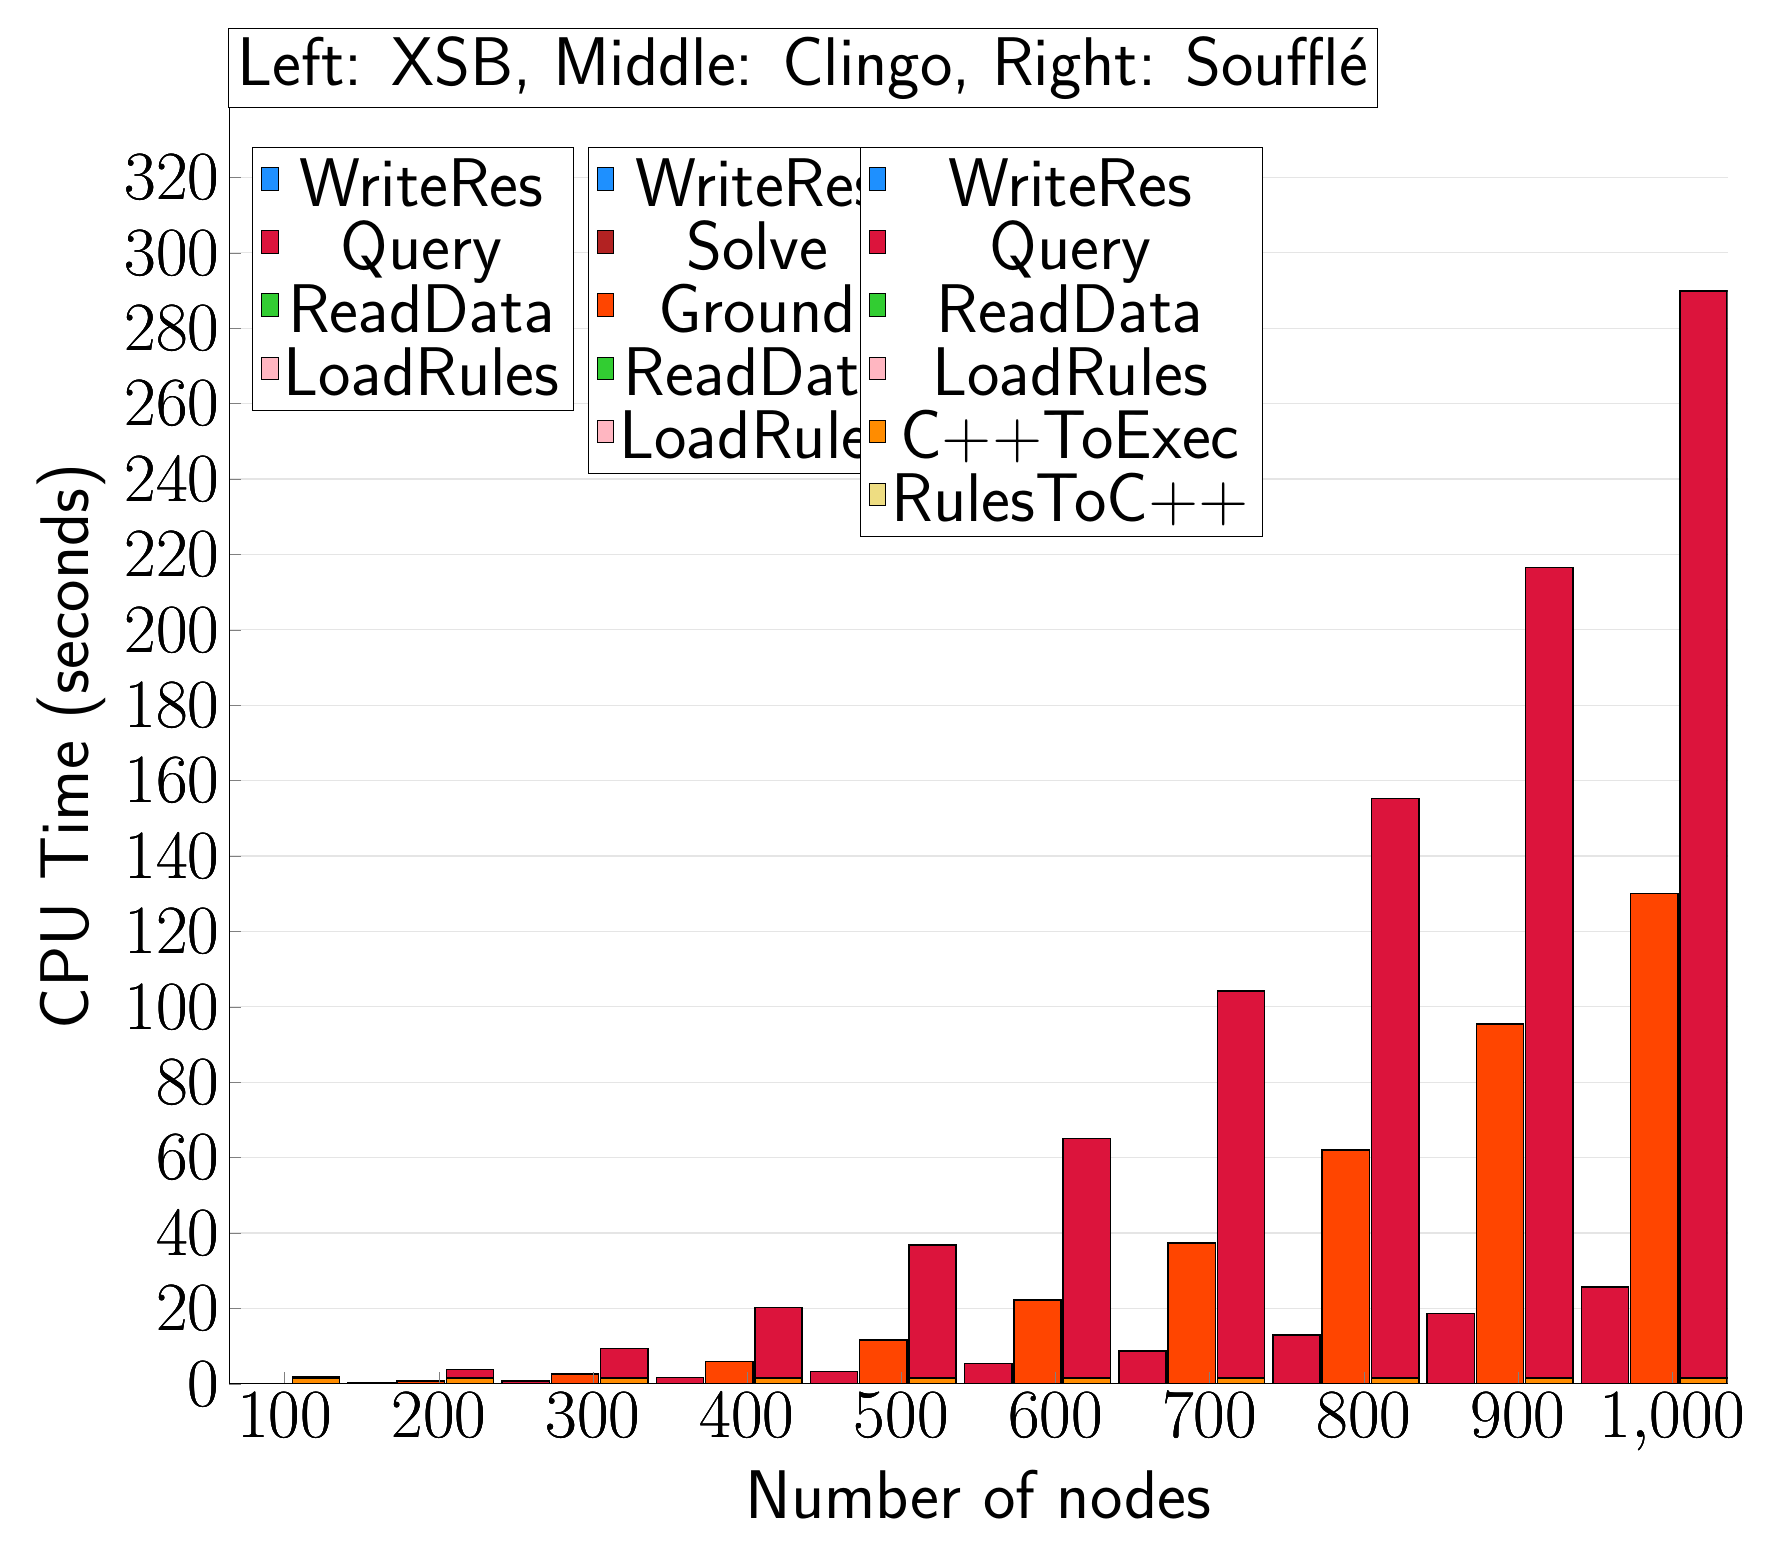
\begin{tikzpicture}
                        \begin{axis}[bar shift=-24.3pt, 
   ybar stacked,
   width=1.7\textwidth,
   bar width=0.6cm,
   ymajorgrids, tick align=inside,
   major grid style={draw=gray!20},
   xtick=data,
   ymin=0, ymax=338.29920000000004,
   axis x line*=bottom,
   axis y line*=left,
   enlarge x limits=0.04,
   legend style={
       at={(0.23, 0.97)},
       anchor=north east,
       legend columns=1,
       font=\Huge,
   },
   ylabel={CPU Time (seconds)},
   xlabel={Number of nodes},
   label style={font=\Huge},
   tick label style={font=\Huge},
]
\addlegendimage{fill=DodgerBlue, draw=black, line width=0.2pt}
\addlegendentry{WriteRes}
\addlegendimage{fill=Crimson, draw=black, line width=0.2pt}
\addlegendentry{Query}
\addlegendimage{fill=LimeGreen, draw=black, line width=0.2pt}
\addlegendentry{ReadData}
\addlegendimage{fill=LightPink, draw=black, line width=0.2pt}
\addlegendentry{LoadRules}
\addplot +[fill=LightPink, draw=black, line width=0.55pt] coordinates {
(100, 0.0005507999999999999)
(200, 0.0005529999999999996)
(300, 0.0005535999999999994)
(400, 0.0005534)
(500, 0.0005582000000000004)
(600, 0.0005502)
(700, 0.0005610000000000001)
(800, 0.0005603999999999997)
(900, 0.0005525999999999997)
(1000, 0.0005565999999999994)
};
\addplot +[fill=LimeGreen, draw=black, line width=0.55pt] coordinates {
(100, 0.00019980000000000003)
(200, 0.0002786000000000002)
(300, 0.0003532000000000004)
(400, 0.0004366000000000002)
(500, 0.0005113999999999996)
(600, 0.0006007999999999996)
(700, 0.0006752000000000003)
(800, 0.0007542)
(900, 0.0008276000000000001)
(1000, 0.0009028000000000003)
};
\addplot +[fill=Crimson, draw=black, line width=0.55pt] coordinates {
(100, 0.0265558)
(200, 0.2104574)
(300, 0.6897865999999999)
(400, 1.6432272)
(500, 3.2305194)
(600, 5.4456698)
(700, 8.6674674)
(800, 12.9998714)
(900, 18.5972262)
(1000, 25.633191)
};
\addplot +[fill=DodgerBlue, draw=black, line width=0.55pt] coordinates {
(100, 6.939999999999933e-05)
(200, -0.000402199999999997)
(300, 0.0005447999999999897)
(400, -0.003816399999999964)
(500, -0.005625400000000003)
(600, -0.009310600000000058)
(700, -0.02427880000000009)
(800, 0.019136199999999447)
(900, 0.033193200000000186)
(1000, 0.06487619999999979)
};
\end{axis}

\begin{axis}[bar shift=-6.5pt, 
   ybar stacked,
   width=1.7\textwidth,
   bar width=0.6cm,
   ymajorgrids, tick align=inside,
   major grid style={draw=none},
   xtick=data,
   ymin=0, ymax=338.29920000000004,
   axis x line*=none,
   axis y line*=none,
   enlarge x limits=0.04,
   legend style={
       at={(0.454, 0.97)},
       anchor=north east,
       legend columns=1,
       font=\Huge,
   },
   label style={font=\Huge},
   tick label style={font=\Huge},
]
\addlegendimage{fill=DodgerBlue, draw=black, line width=0.2pt}
\addlegendentry{WriteRes}
\addlegendimage{fill=FireBrick, draw=black, line width=0.2pt}
\addlegendentry{Solve}
\addlegendimage{fill=OrangeRed, draw=black, line width=0.2pt}
\addlegendentry{Ground}
\addlegendimage{fill=LimeGreen, draw=black, line width=0.2pt}
\addlegendentry{ReadData}
\addlegendimage{fill=LightPink, draw=black, line width=0.2pt}
\addlegendentry{LoadRules}
\addplot +[fill=LightPink, draw=black, line width=0.55pt] coordinates {
(100, 0.0)
(200, 0.0)
(300, 0.0)
(400, 0.0)
(500, 0.0)
(600, 0.0)
(700, 0.0)
(800, 0.0)
(900, 0.0)
(1000, 0.0)
};
\addplot +[fill=LimeGreen, draw=black, line width=0.55pt] coordinates {
(100, 0.0)
(200, 0.0)
(300, 0.0)
(400, 0.0)
(500, 0.0020000000000000018)
(600, 0.0)
(700, 0.0)
(800, 0.0)
(900, 0.0)
(1000, 0.001999999999999996)
};
\addplot +[fill=OrangeRed, draw=black, line width=0.55pt] coordinates {
(100, 0.11000000000000001)
(200, 0.728)
(300, 2.624)
(400, 5.952)
(500, 11.642)
(600, 22.266)
(700, 37.396)
(800, 62.022000000000006)
(900, 95.47)
(1000, 130.048)
};
\addplot +[fill=FireBrick, draw=black, line width=0.55pt] coordinates {
(100, 0.0)
(200, 0.0)
(300, 0.0)
(400, 0.0)
(500, 0.003999999999999915)
(600, 0.0)
(700, 0.001999999999999602)
(800, 0.003999999999999204)
(900, 0.001999999999998181)
(1000, 0.002000000000001023)
};
\addplot +[fill=DodgerBlue, draw=black, line width=0.55pt] coordinates {
(100, 0.0020000000000000018)
(200, 0.0)
(300, 0.0)
(400, 0.0)
(500, -0.0019999999999999575)
(600, 0.0)
(700, -0.001999999999999602)
(800, -0.003999999999999204)
(900, 0.002000000000001023)
(1000, -0.002000000000001023)
};
\end{axis}

\begin{axis}[bar shift=11.3pt, 
   ybar stacked,
   width=1.7\textwidth,
   bar width=0.6cm,
   ymajorgrids, tick align=inside,
   major grid style={draw=none},
   xtick=data,
   ymin=0, ymax=338.29920000000004,
   axis x line*=none,
   axis y line*=none,
   enlarge x limits=0.04,
   legend style={
       at={(0.69, 0.97)},
       anchor=north east,
       legend columns=1,
       font=\Huge,
   },
   label style={font=\Huge},
   tick label style={font=\Huge},
]
\addlegendimage{fill=DodgerBlue, draw=black, line width=0.2pt}
\addlegendentry{WriteRes}
\addlegendimage{fill=Crimson, draw=black, line width=0.2pt}
\addlegendentry{Query}
\addlegendimage{fill=LimeGreen, draw=black, line width=0.2pt}
\addlegendentry{ReadData}
\addlegendimage{fill=LightPink, draw=black, line width=0.2pt}
\addlegendentry{LoadRules}
\addlegendimage{fill=DarkOrange, draw=black, line width=0.2pt}
\addlegendentry{C++ToExec}
\addlegendimage{fill=LightGoldenrod, draw=black, line width=0.2pt}
\addlegendentry{RulesToC++}
\addplot +[fill=LightGoldenrod, draw=black, line width=0.55pt] coordinates {
(100, 0.008000000000000002)
(200, 0.006000000000000001)
(300, 0.010000000000000002)
(400, 0.006000000000000001)
(500, 0.004000000000000001)
(600, 0.0020000000000000005)
(700, 0.004000000000000001)
(800, 0.0020000000000000005)
(900, 0.0)
(1000, 0.0)
};
\addplot +[fill=DarkOrange, draw=black, line width=0.55pt] coordinates {
(100, 1.52)
(200, 1.53)
(300, 1.5220000000000002)
(400, 1.52)
(500, 1.528)
(600, 1.518)
(700, 1.518)
(800, 1.518)
(900, 1.52)
(1000, 1.5220000000000002)
};
\addplot +[fill=LightPink, draw=black, line width=0.55pt] coordinates {
(100, 0.00017759999999999998)
(200, 0.00016360000000000002)
(300, 0.0001526)
(400, 0.000158)
(500, 0.00015600000000000002)
(600, 0.0001626)
(700, 0.00016460000000000002)
(800, 0.0001732)
(900, 0.0001654)
(1000, 0.00016839999999999997)
};
\addplot +[fill=LimeGreen, draw=black, line width=0.55pt] coordinates {
(100, 0.0008738000000000001)
(200, 0.0012214)
(300, 0.0016288000000000001)
(400, 0.0020603999999999996)
(500, 0.0022374)
(600, 0.0028224)
(700, 0.0032372000000000004)
(800, 0.0035872)
(900, 0.0039324)
(1000, 0.0043104)
};
\addplot +[fill=Crimson, draw=black, line width=0.55pt] coordinates {
(100, 0.303342)
(200, 2.299058)
(300, 7.772150000000001)
(400, 18.77584)
(500, 35.29434)
(600, 63.59358000000001)
(700, 102.60619999999999)
(800, 153.7144)
(900, 214.94700000000003)
(1000, 288.29920000000004)
};
\addplot +[fill=DodgerBlue, draw=black, line width=0.55pt] coordinates {
(100, 0.00027020000000000006)
(200, 0.0003764)
(300, 0.00043119999999999996)
(400, 0.00037099999999999996)
(500, 0.0004332)
(600, 0.00038800000000000005)
(700, 0.0004084)
(800, 0.0004398)
(900, 0.0004963999999999999)
(1000, 0.00042259999999999997)
};
\end{axis}


\node[anchor=south, draw, fill=white] at (rel axis cs:0.42,1) {\Huge Left: XSB, Middle: Clingo, Right: Soufflé};
\end{tikzpicture}
\end{document}
                    